% ============================================================================
% SECTION 0: DOCUMENT CLASS AND PREAMBLE
% ============================================================================
\documentclass[12pt, letterpaper]{report}% "letterpaper" matches US standard paper size.
\setcounter{tocdepth}{3}
% --- PACKAGES: Each one adds a capability to LaTeX ---
% Think of packages like Python imports or C #includes.


% Manual change 

% ---------- Page Layout ----------
\usepackage[top=1in,bottom=1in,left=1in,right=1in]{geometry} % geometry lets you set margins. 1-inch all around is standard for reports.
% ---------- Encoding & Fonts ----------
\usepackage[utf8]{inputenc}% Allows special characters (é, ü, °) to be typed directly.
\usepackage[T1]{fontenc} % Ensures proper font encoding in the output PDF. Without this, copy-pasting from the PDF can produce garbled characters.
% ---------- Graphics & Figures ----------
\usepackage{graphicx}% THE core package for inserting images.
% Usage: \includegraphics[width=0.8\textwidth]{filename.png}
\graphicspath{{figures/}}
\usepackage{float}% Gives you the [H] placement option for figures/tables. [H] means "put it HERE, not where LaTeX thinks is best." Very useful when you need a figure right after the text that references it.
\usepackage{subcaption}% Lets you put multiple images side-by-side in a single figure environment. Example: Figure 3(a) and Figure 3(b) next to each other.
% ---------- Tables ----------
\usepackage{booktabs} % Provides \toprule, \midrule, \bottomrule for professional-looking tables.
% Rule of thumb: NEVER use vertical lines in tables. Use booktabs rules instead.
\usepackage{tabularx}% Adds the tabularx environment, which lets columns auto-expand to fill width. Great for tables that need to span the full page width.
\usepackage{multirow}% Allows cells that span multiple rows in tables.
\usepackage{longtable}% For tables that are too long to fit on one page (like a Bill of Materials).
% ---------- Math ----------
\usepackage{amsmath}% The standard package for equations. Adds align, equation*, etc.
\usepackage{amssymb}% Extra math symbols (e.g., \therefore, \because, \pm).
\usepackage{siunitx}% Proper formatting for SI units.
% Usage: \SI{100}{\celsius}, \SI{10000}{psi}, \SI{10}{\centi\meter}
% This ensures consistent unit formatting throughout the document.
% ---------- Cross-Referencing & Links ----------
\usepackage[
    colorlinks=true,
    linkcolor=blue,      % Internal links (sections, figures)
    citecolor=blue,      % Citation links
    urlcolor=blue         % URL links
]{hyperref}
% Makes all references, citations, and URLs clickable in the PDF.
% Set colorlinks=false if you want boxes instead of colored text.
% ---------- Bibliography ----------
\usepackage[numbers, sort&compress]{natbib}
% IEEE-style numeric citations: [1], [2,3], [4-7]
% "sort&compress" turns [3,1,2] into [1-3]
% ---------- Captions ----------
\usepackage[
    font=small,           % Caption text slightly smaller than body
    labelfont=bf,         % "Figure 1:" is bold
    textfont=it            % The caption description is italic
]{caption}% Makes figure/table captions look more professional.
% ---------- Headers & Footers ----------
\usepackage{fancyhdr}% Customizable headers and footers.
\pagestyle{fancy}% Activate the fancy header/footer style.
\fancyhf{}% Clear all default header/footer content.
\fancyhead[L]{\small Team 16 --- Noble Aggie Labs}% Left header: team name.
\fancyhead[R]{\small EME 185}% Right header: course number.
\fancyfoot[C]{\thepage}% Center footer: page number.
\renewcommand{\headrulewidth}{0.4pt}% Thin line under the header. Set to 0pt to remove.
% ---------- Paragraph Formatting ----------
\usepackage{parskip}% Adds space between paragraphs instead of indenting the first line. This is more common in engineering reports than academic papers.
\setlength{\parindent}{0pt}% Explicitly remove paragraph indentation (parskip should handle this, but belt-and-suspenders doesn't hurt for readability).
% ---------- Line Spacing ----------
\usepackage{setspace}
\onehalfspacing% 1.5 line spacing is easier to read and mark up than single spacing. Change to \doublespacing if required.
%-------- For Box diagrams
\usepackage{tikz}
\usetikzlibrary{arrows.meta, positioning}
% ---------- Appendix Support ----------
\usepackage[toc, page]{appendix} % Adds "Appendices" header and includes appendices in the Table of Contents.
%----------- Title/Chapter formatting -----------------
\usepackage{titlesec}
% Format \chapter to look simple (no giant text, no separate page)
\titleformat{\chapter}
  {\LARGE\bfseries}  % format
  {}                % label
  {0em}                         % sep between label and title
  {}                            % before-code
\titlespacing*{\chapter}{0pt}{20pt}{10pt}  % left, before, after
% ---------- PDF Metadata ----------
\hypersetup{
    pdftitle={Preliminary Machine Architecture Report -- Passive Temperature Compensation Device},
    pdfauthor={Team 16: Noble Aggie Labs},
    pdfsubject={EME-185A/B Senior Design, UC Davis},
}


% ============================================================================
% SECTION 0.5: CUSTOM COMMANDS (Modular Helpers)
% ============================================================================
% These are reusable shortcuts. Define them once, use them everywhere.
% If a name or term changes, you only edit it in ONE place.

% --- Project-specific shortcuts ---
\newcommand{\projecttitle}{Passive Temperature Compensation Device}
\newcommand{\teamname}{Noble Aggie Labs}
\newcommand{\teamnumber}{16}
\newcommand{\sponsor}{Dr.\ Bradley Bon}
\newcommand{\organization}{Sandia National Laboratories}
\newcommand{\coursename}{EME 185}
\newcommand{\instructor}{Professor Jonathan Schofield}
\newcommand{\ta}{Xiangpu Wang}
\newcommand{\duedate}{16 March 2026}
% --- Convenience commands for common terms ---
% Using these ensures consistent terminology throughout the report.
\newcommand{\device}{PTCD}
\newcommand{\tcd}{TCD}              % Temperature Compensation Device
\newcommand{\degC}{^{\circ}C}    % Degree Celsius symbol, properly formatted
\newcommand{\psid}{\text{psid}}      % Pressure differential unit
\newcommand{\sbsInterface}{Interface}
\newcommand{\sbsValve}{Valve Mechanism}
\newcommand{\sbsActuator}{Actuator}
\newcommand{\requiredRelationship}{D_{\text{effective}} = A_1 (T_{\text{ambient}} - T_{\text{reference}}) + A_0}
\newcommand{\govActuator}{\Delta L = L_0 \Delta T \alpha}
\newcommand{\govInterface}{\Delta S = \frac{R}{r}\Delta L}
\newcommand{\govValve}{D_{\text{eff}} = \sqrt{\frac{2}{pi}}}
\newcommand{\thermalStress}{\Delta L = L_0 \int \alpha(T)\, dt} %idk
\newcommand{\specTempHigh}{80} %Celcius
\newcommand{\specTempLow}{-60} %Celcius
\newcommand{\specTempRef}{25} %Celcius
\newcommand{\specVol}{10} % Maximum volume in cm^3
\newcommand{\specPressure}{68.94757}%MPa
\newcommand{\specDeffLow}{0.17018} %mm
\newcommand{\specDeffHigh}{0.38354} %mm
\newcommand{\specTolerancePercent}{\pm 5\%}
\newcommand{\specDeffConstOne}{-1.524(10)^{-3}} %mm/degC
\newcommand{\specDeffConstTwo}{0.254} %mm
\newcommand{\specStroke}{0.01053} %inch
\newcommand{\specPressureForceAxial}{placeholderaxialforce} % N
\newcommand{\specActuatorMateria}{placeholderactuatormaterial} % No units
\newcommand{\specActuatorCTE}{placeholderCTEvalueactuator} % 10^-6/ºC

% --- Figure insertion helper ---
% This command simplifies inserting a figure with a caption and label.
% Usage: \insertfigure{width}{filename}{caption text}{fig:label}
%
% Parameters:
%   #1 = width relative to text width (e.g., 0.8 for 80%)
%   #2 = filename (without path if images are in the same directory)
%   #3 = caption text
%   #4 = label for cross-referencing (use fig: prefix by convention)
\newcommand{\insertfigure}[4]{%
    \begin{figure}[H]
        \centering
        \includegraphics[width=#1\textwidth]{#2}
        \caption{#3}
        \label{#4}
    \end{figure}
}

% --- TODO marker for draft mode ---
% Prints a bold red "TODO" so you can easily spot incomplete sections.
\usepackage{xcolor}
\newcommand{\todo}[1]{{\bfseries\color{red}[TODO: #1]}}


% ============================================================================
% BEGIN DOCUMENT
% ============================================================================
\begin{document}
\begin{titlepage}
    \thispagestyle{empty}   % No header/footer on the title page

    % --- Cover Photo: Sandia National Laboratories Aerial View ---
    \begin{center}
        % TODO: Uncomment the next line and provide the correct filename
        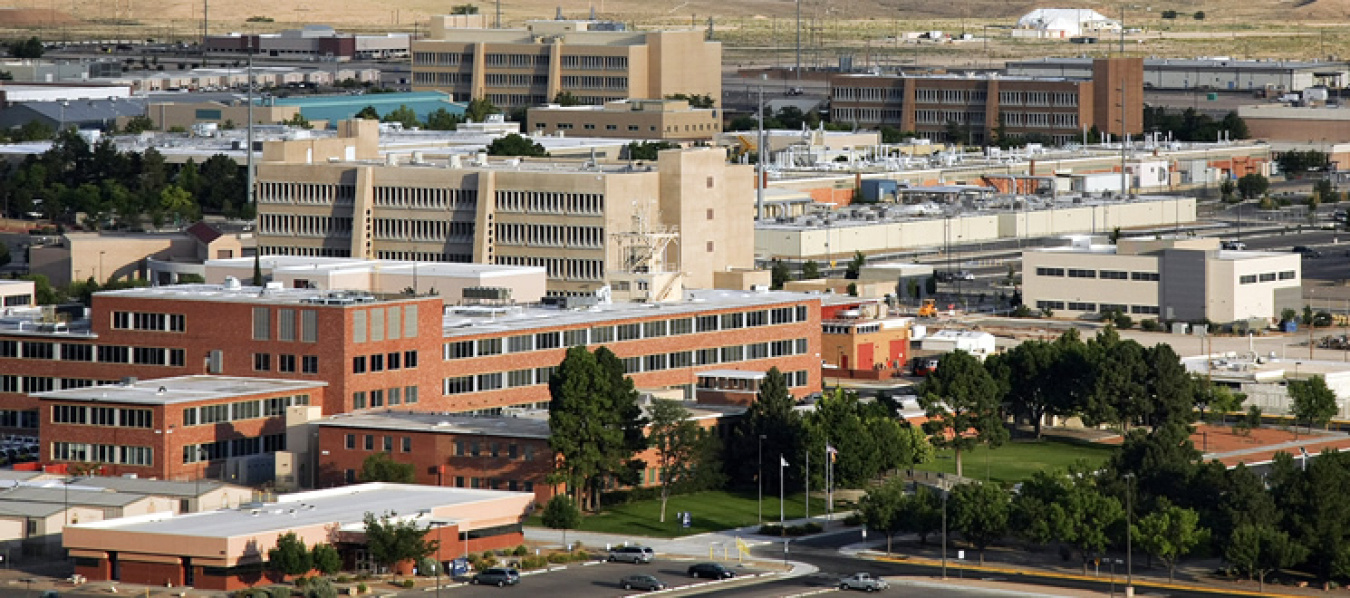
\includegraphics[width=\textwidth]{SandiaNationalLabCoverPhoto2.jpg}
        % Placeholder rectangle if image is not yet available:
    \end{center}
    \vspace{0.4in}
    % --- UC Davis College of Engineering Logo ---
    \begin{center}
        % TODO: Uncomment and provide the correct filename
        % \includegraphics[height=1in]{ucdavis_coe_logo.png}

        % Placeholder if logo not yet available:
        {\Large\bfseries\color{blue!70!black} UC\,DAVIS}\\[2pt]
        {\normalsize\scshape College of Engineering}
    \end{center}
    \vspace{0.6in}
    % --- Project Title ---
    \begin{center}
        {\LARGE\bfseries\color{blue!70!black} \projecttitle}\\[12pt]
        {\large\bfseries SPONSORED BY: \MakeUppercase{\sponsor, \organization}}
    \end{center}
    \vfill  % Push the following content to the vertical center/bottom

    % --- Report Type ---
    \begin{center}
        {\large\bfseries PRELIMINARY MACHINE ARCHITECTURE REPORT}
    \end{center}

    \vspace{0.4in}

    % --- Course Information ---
    \begin{center}
        {\large \coursename}\\[4pt]
        {\large \MakeUppercase{\instructor}}\\[4pt]
        {\large \MakeUppercase{\ta, Teaching Assistant}}
    \end{center}

    \vspace{0.4in}

    % --- Submission Deadline ---
    \begin{center}
        {\large\bfseries SUBMISSION DEADLINE: \MakeUppercase{\duedate}}
    \end{center}

    \vspace{0.5in}
\end{titlepage}


% ============================================================================
% TEAM MEMBER PAGE
% ============================================================================
% This page lists all team members, as shown in the Report 2 Template.
% The grading rubric (Section I) checks that all names are present.
% ============================================================================

\newpage
\thispagestyle{empty}  % No header/footer on this page either

\vspace*{1in}
\begin{center}
    {\Large\bfseries Team \teamnumber}\\[24pt]

    % --- List all team members ---
    % TODO: Verify spelling of all names
    {\large
        Isaiah Mathew\\[8pt]
        Jon Pizarro\\[8pt]
        Nicholas Metta\\[8pt]
        John Bodine\\[8pt]
        Miguel Cuaycong\\[8pt]
        Sam van der Veen\\[8pt]
    }

    \vspace{0.8in}

    {\Large\itshape \projecttitle}\\[12pt]
    {\large By the}\\[12pt]
    {\Large\bfseries \teamname}\\[24pt]
    {\large Sponsored by \sponsor, \organization}\\[36pt]
    {\large Preliminary Machine Architecture Report}\\[12pt]
    {\large \coursename}\\[6pt]
    {\large \instructor}\\[6pt]
    {\large TA \ta}\\[12pt]
    {\large Due \duedate}
\end{center}


% ============================================================================
% TABLE OF CONTENTS
% ============================================================================
% GRADING: Section 1.3 — 5.0 points
%   "Accurate page numbers, headings and sub-headings used"
%
% LaTeX generates this automatically from \section and \subsection commands.
% You MUST compile TWICE for page numbers to update correctly.
% ============================================================================

\newpage
\tableofcontents
\listoffigures
\listoftables

\newpage  % Start the body of the report on a fresh page

\chapter{Abstract}
\label{sec:abstract}

%--- BEGIN CONTENT ---

% PARGRAPH 1: Project objective and motivation
Sandia National Laboratories (SNL) has tasked our senior design team, 
\teamname\ to design a passive temperature compensation device (\device) that regulates flow in a pipe. 
Flow must be regulated by adjusting an orifice geometry according to a change in ambient air temperature.
The \device\ must be purely thermo-mechanically driven, functioning without the reliance on embedded systems(electronics) or human input.
The required mathematical relationship between the ambient temperature and a characteristic orifice geometry is provided by SNL.
Additionally, materials compatibility with the fluid --primarily noble gases-- must be considered.
In order to meet these requirements, the \device\ will be divided into three main subsystems: (1) \sbsActuator, (2) \sbsInterface, (3) \sbsValve.

% PARAGRAPH 2: Solution and progress to date
This Preliminary Machine Architecture Report outlines how well the current iteration of the three main subsystems conform to the specified mathematical relationship.
Explicitly, the relationship between the orifice diameter and the ambient temperature can be summarized as $\requiredRelationship$\ which will be referred to as the "required relationship" throughout this report.
The \device\ and its constituent subsystems must facilitate this linear relationship between the characteristic orifice diameter and the ambient temperature. 
\todo{Talk about sealing(bellows)}



\chapter{System Architecture}
\label{sec:system_architecture}

% --- 2.1: Selection Criteria and Justification ---
% WHY this design? Focus on positive attributes.
% Reference your concept screening/scoring matrices (Appendix).

    \begin{figure}[H]
        \centering
        % \includegraphics[width=0.85\textwidth]{system_assembly_isometric.png}

        % Placeholder:
        \fbox{\parbox[c][3in]{0.85\textwidth}{%
            \centering\Large%
            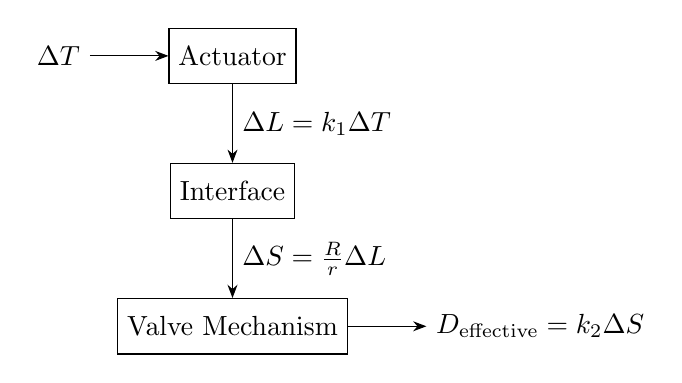
\begin{tikzpicture}[
                block/.style={draw, rectangle, minimum height=2em, minimum width=4em},
                sum/.style={draw, circle, inner sep=0pt, minimum size=6mm},
                >=Stealth
            ]

                \node[block] (interface)                        {\sbsInterface};
                \node[block] (actuator) [above = of interface]  {\sbsActuator};
                \node[block] (valve)    [below = of interface]  {\sbsValve};

                \node(temp_input)   [left = of actuator]   {$\Delta T$};
                \node(diam_output)  [right = of valve]      {$D_{\text{effective}} = k_2 \Delta S$};

                \draw[->] (temp_input) -- (actuator);
                \draw[->] (valve) -- (diam_output);
                \draw[->] (actuator) to node[right] {$\Delta L = k_1 \Delta T$} (interface) ;
                \draw[->] (interface) to node[right] {$\Delta S = \frac{R}{r} \Delta L$} (valve);

            \end{tikzpicture}
        }   
    }

        \caption{Controls diagram of the  \device. Outlines the overall flow of inputs
        and outputs across the subsystems.}
        \label{fig:controls_diagram}
    \end{figure}

    \begin{figure}[H]
        \centering
        % \includegraphics[width=0.85\textwidth]{system_assembly_isometric.png}

        % Placeholder:
        \fbox{
            \parbox[c][3in]{0.85\textwidth}{%
            \centering\Large%
            }   
        }

        \caption{Exploded View}
        \label{fig:explodedoverall}
    \end{figure}

    \begin{table}[H]
        \centering
        \caption{Overall requirements and specifications summary}
        \label{tab:requirements and specification}
        \begin{tabularx}{\textwidth}{l X l}
            \toprule
            \textbf{Requirements} & \textbf{Spec} & \textbf{Subsystem Rolldown} \\
            \midrule
            Temp.\ range &
            \specTempLow $\degC$\ to \specTempHigh $\degC$ &
            \sbsActuator
            \\\addlinespace
            Mech.\ envelope &
            $\leq$ \specVol\ cm$^3$ &
            Entire device
            \\\addlinespace
            Pressure &
            $\Delta P \leq 68.95$~MPa &
            \sbsValve
            \\\addlinespace
            Eff.\ diameter &
            $D_{\text{eff}}$ = 0.170--0.384~mm & 
            \sbsValve
            \\\addlinespace
            Tolerance &
            $D_{\text{eff}}$ = $\pm 0.0127$~mm & 
            Entire device
            \\\addlinespace
            Fluid compatibility &
            "High" free energy of reaction with noble gas &
            \sbsValve
            \\\addlinespace
            Sealing/Fluid diffusion &
            TODO: Quantify seal quality somehow &
            \sbsValve\ and \sbsInterface
            \\\bottomrule
        \end{tabularx}
    \end{table}
    \section{Selection criteria}
    % Paragraph 1: Criteria Choice Established
    Since the preliminary design report, every subsystem decision has deviated since. After many iterations of designing and consulting with professionals,
    our team selected the final design for each subsystem based on the following criteria:

    \begin{enumerate}
        \item Linearity. The required relationship to hold the orifice geometry must be linear. As such, each susbsystem design preserves
        this linear relationship by having a governing equation that ensures a linear input-output relationship. Each of our previous designs were at least second order if not higher
        order. Therefore, choosing a design with this linear relationship became the impetus for our current design decisions.
        \item Hydrogen compability. Since hydrogen or potentially other noble gases will be the working fluid, we chose a design that has no polymers,
        elastomers, or permeable seals present in the flow path. The chosen "pizza cutter valve" meets the material requirements and design requirements
        to be hydrogen compatible. 
        \item Manufacturability. When thinking of the constraings for the design, we equally thought of the constraints to manufacture. We chose the current designs with this in mind. 
        For instance, the valve is a single moving plate. The actuator is a single moving rod. While the size of these parts with respect to the mechanical envelope is a challenge in it of itself,
        they avoid complex moving parts such as gear trains. 
        \item Thermal isolation. The actuator rod is separated by the gas using the housing walls and bellows. The actuation signal responds to ambient temperature instead of the gas temperature.
        With this design choice we can ensure a lack of heat transfer between the valve and the actuator that could otherwise impact performance. 
        \item Pressure integrity. To meet the strenuous pressure requirement, we chose Inconel 718 bellows, a actutaor, and an all-metal housing that should withstand the 68.95 MPa of pressure.
    \end{enumerate}

    % Paragraph 2: Actuator Design Choice Explained
    In the first preliminary design report, the bimetallic thermal expansion rod was chosen as the actuator. However, it was later overruled for one critical reason: it could extend to the required amount needed
    to actuate the valve without violating the mechanical envelope. After more discussion, we considered pursuing the gas piston cylinder. However, after extensive design two flaws made this design also obsolete. Firstly,
    the gas piston cylinder was impossible to hermetically seal. Secondly, the overcoming the friction????  As such, we looked towards using thermal expansion to actuate the valve since any device that relies on thermal
    expansion as the mechanism is inherently hermetically sealed and has significantly less moving parts than something like a piston cylinder. We've chosen a singular $placeholderactuatormaterial$ thermal expansoin rod as our design choice.

    The actuator relies on thermal expansion of a single metallic rod whose change in length is governed by the following equation: $\govActuator$. This relationship can only be maintained as linear provided that the thermal
    expansion constant $\alpha$ remains approximately constant throughout the operating temperature range. $placeholderactuatormaterial$ alloys exhibit at CTE of $placeholderCTEvalueactuator$, which varies by less than some percentage between
    -60$\degC$ to -80$\degC$. This is well within the tolerance permitted by the $\pm$5\% uncertainty in $A_1$. 

    % Paragraph 3: Actuator Advantages
    This section discusses the advantages of the singular rod design.
    \begin{enumerate}
        \item The singular thermal expansion rod is mechanically simple. There are no bonded interfaces, no internal fluids, no phase transitions unlike the gas piston cylinder. Moreover, the design has no failure modes with delamination (bimetallic coils), non-linear volumetric expansion (wax piston), or gas leakage (gas piston cylinder).
        \item The rod is entirely metallic and hydrogen-compatible. It satisfies the material requirment as there are no polymers. Most importantly, however, the rod is thermally isolated from the gas flow. The 20$\degC$ maximum temperature difference between the gas and ambient air does not corrupt the actuation process.
        \item The rod can generated substantial force under constraint. The thermal stress formula: $\thermalStress$ shows forces on the order of several hundred newtons. This is quite impressive as the diamter of the actuator is quite small. This suggests that the actuator is more than capable of overcoming the spring forces of the bellows. Overall, this reinforces that the the system will actuate relaibly across the entire temperature range without failure. 
    \end{enumerate}

    % Paragraph 4: Valve Design Choice Explained
    The chosen design choice for the valve is redfined version of the hexagonal aperature. The new valve design is a mechanism that consists of two flate plates--one fixed and one translating, each containing an identical rectangualr slot in the center. The plates are held in surface contact such that the overlap of the two slots defines the flow orifice.
    When the actuator extends with increasing temperature, the overlap area is reduced and shrinks $D_eff$ as required. The overlap of these two identical triangles are offset vertically by a distance x. The design choice forms a rhombus. The area of that rhombus is critical as it depends linearly on that plate offset. It is this exact relationship that led us to choosing this as the primary design choice.
    It is the only valve design that has a neat linear relationship to our knowledge. %insert linear relationship explanation and calculations

    We ultimately selected the valve architecture over the hexagonal diaphragm for three main reasons:
    \begin{enumerate}
        \item Manufacturability. The sliding-plate design has only one moving part, which is the translating plate. This is abundantly simpler than the six interlocking trapezoidal blades of the hexagonal diaphragm. This reduces manufacting complexity and the number of interfaces where leakage could occur.
        \item Linearity. As stated previously, the governing equation of the sliding-plate valve is the only valve design with a linear relationship. Every other valve design has at least a difference of squares if not higher order terms. This is a necessary design constraint that only the sliding-plate meets. 
        \item Size. The sliding-plate can fit within the 10 $cm^3$ mechanical envelope. The hexagonal aperature was too complex to manufacture given its size. Moreover, after computing the necessary dimensions to determine functionality. The hexagonal aperature would need to be larger than the mechanical envelope to function as intended.
    \end{enumerate}
        \todo{Well defined requirements, design and requirements related, subsystem selection is clear}
    \section{Subsystem Overview}
    \todo{This is where the description of the system architecture goes}

    


        \todo{Clean up the following paragraphs or move to discussion}
        The relationship between the ambient temperature and its corresponding orifice geometry is governed by the following equation:

        \begin{equation}
            \requiredRelationship
            \label{eq: required_relationship}
        \end{equation}

        Where:
        \begin{align*}
            &A_1 = \specDeffConstOne \specTolerancePercent\ \frac{\text{mm}}\degC
            \\
            &A_0 = \specDeffConstTwo \specTolerancePercent\ \text{mm}
            \\
            &T_{\text{ref}} = \specTempRef \degC
            \\
            &T_{ambient}\ \epsilon\ [\specTempLow, \specTempHigh] \degC 
        \end{align*}
        (1)~a \textbf{aluminum thermal expansion rod} a singular metallic rod that responds to ambient temperature changes. 
        The aluminum rod will have linear piston displacement as a result of thermal exapnsion via the following equation:

        \begin{equation}
            \Delta L = L_0\,\Delta T\, \alpha\
        \end{equation}

        (2)~A \textbf{compound spur-gear train} comprising of two rack gears and two coaxial pinion gears with a gear ratio of
        4:1. This amplifies and transmits the piston's linear motion to the valve; and 
        (3)~a \textbf{sliding-plate orifice valve} (''pizza cutter'' design), in which two flat plates, one fixed and one translating
        contain a shaped hole with the overlap between the two holes defining the effective flow orifice. As the actuator extends with 
        increasing temperature, the moving plate translates downwards. This reduces the overlap area and shriking $D_{\text{eff}}$ per 
        the requirements. 

%--- END CONTENT ---


% --- 2.2: System Overview with Figures ---
% Show the WHOLE system first, then break into subsystems.

% ============================================================================
% SECTION 3: DISCUSSION
% ============================================================================
% GRADING: Section IV — 25 points total
%   4.1) Discussion of requirements and rolldown to subsystems (5.0 pts)
%        "Half points well described requirement updates,
%         half points roll down discussion"
%   4.2) Discussion of subsystem interactions (10.0 pts)
%        "Half marks accurate technical discussions, describes how
%         subsystems work together. Half marks for proper engineering
%         drawing package."
%   4.3) Proof that design will meet requirements / calculations (10.0 pts)
%        "Accurate, well motivated / related to requirements,
%         reasonable assumptions stated"
%
% This is the MOST HEAVILY WEIGHTED section (25 pts).
% ============================================================================

\chapter{Discussion}
\label{sec:discussion}
    %--- BEGIN CONTENT ---
    \section{Valve}
        \begin{table}[H]
            \centering
            \caption{Valve Specifications}
            \label{tab:valve specification}
            \begin{tabularx}{\textwidth}{l X l}
                \toprule
                \textbf{Requirements} & \textbf{Design Specification} & \textbf{Implemented Specification} \\
                \midrule
                Mech.\ envelope &
                $\leq$ \specVol\ cm$^3$ &
                TODO: Insert volume of mechanism
                \\\addlinespace
                Pressure &
                $\Delta P \leq 68.95$~MPa &
                TODO: Insert FOS or necessary par.
                \\\addlinespace
                Eff.\ diameter &
                $D_{\text{eff}}$ = 0.170--0.384~mm & 
                TODO: Insert orifice geometry
                \\\addlinespace
                Tolerance &
                $D_{\text{eff}}$ = $\pm 0.0127$~mm & 
                TODO: Insert orifice geometry
                \\\addlinespace
                Fluid compatibility &
                "High" free energy of reaction with noble gas &
                TODO: Insert material prop.
                \\\addlinespace
                Sealing/Fluid diffusion &
                TODO: Quantify seal quality somehow &
                TODO: Insert corresponding spec
                \\\bottomrule
            \end{tabularx}
        \end{table}
        \subsection{Orifice}
            \subsubsection{Design Requirement Updates}
            \label{subsec:req_updates}

            \subsubsection{Current Implementation} 
            
                \begin{figure}[H]
                    \centering
                    % \includegraphics[width=0.85\textwidth]{system_assembly_isometric.png}

                    % Placeholder:
                    \fbox{
                        \parbox[c][3in]{0.85\textwidth}{%
                        \centering\Large%
                        }   
                    }

                    \caption{CAD model of the orifice}
                    \label{fig:orifice}
                \end{figure}
                \begin{table}[H]
                    \centering
                    \caption{Valve Specifications}
                    \label{tab:valve specification}
                    \begin{tabularx}{\textwidth}{l X l}
                        \toprule
                        \textbf{Requirements} & \textbf{Design Specification} & \textbf{Implemented Specification} \\
                        \midrule
                        Mech.\ envelope &
                        $\leq$ \specVol\ cm$^3$ &
                        TODO: Insert volume of mechanism
                        \\\addlinespace
                        Pressure &
                        $\Delta P \leq 68.95$~MPa &
                        TODO: Insert FOS or necessary par.
                        \\\addlinespace
                        Eff.\ diameter &
                        $D_{\text{eff}}$ = 0.170--0.384~mm & 
                        TODO: Insert orifice geometry
                        \\\addlinespace
                        Tolerance &
                        $D_{\text{eff}}$ = $\pm 0.0127$~mm & 
                        TODO: Insert orifice geometry
                        \\\addlinespace
                        Fluid compatibility &
                        "High" free energy of reaction with noble gas &
                        TODO: Insert material prop.
                        \\\bottomrule
                    \end{tabularx}
                \end{table}

                The orifice is the critical piece of this design. In order to follow the relationship required by Equation 1, 
                the orifice geometry must drive the rest of the design. Each plate, one fixed and one whose movement is controlled by the actuator, 
                will contain identical rectangular holes near its center. The plates must maintain surface contact such that the overlap between the two holes creates the desired orifice. 
                As the ambient temperature rises, the actuator expands, lowering the moving plate. Because its hole is below that of the fixed plate, the resulting orifice shrinks.
    \subsection{Chassis/Housing}
        \subsubsection{Design Requirement Updates}
        \subsubsection{Current Implementation}

        The valve housing must withstand internal pressure without failing.
        The housing is modeled as a thick-walled cylinder in order to determine the appropriate wall thickness required to sustain the internal pressure.
        The thickness $t$ of the housing is defined as the shortest distance from the inner wall to the outer wall.
        The following equations are used to verify structural integrity under the specified conditions.
        The housing consists of three distinct sections: the inlet, the outlet, and the central body, each of which is analyzed for its ability to withstand the internal pressure.
        Since internal pressure constitutes the only significant structural load, external forces on the housing are neglected.

        Principal Stresses:
        $$\sigma_{\theta} = P \left( \frac{r_o^2 + r_i^2}{r_o^2 - r_i^2} \right) = 68.95 \left( \frac{22.84^2 + 12.7^2}{22.84^2 - 12.7^2} \right) = 68.95 \left( \frac{521.67 + 161.29}{521.67 - 161.29} \right) \approx 130.6 \ \text{MPa} \quad (\text{Hoop Stress})$$
        $$\sigma_{r} = -P = -68.95 \ \text{MPa} \quad (\text{Radial Stress})$$
        $$\sigma_{z} = P \left( \frac{r_i^2}{r_o^2 - r_i^2} \right) = 68.95 \left( \frac{161.29}{360.38} \right) \approx 30.8 \ \text{MPa} \quad (\text{Longitudinal Stress})$$
        \\~\\
        Von Mises Equivalent Stress:
        $$\sigma_{vm} = \sqrt{\frac{(\sigma_\theta - \sigma_r)^2 + (\sigma_r - \sigma_z)^2 + (\sigma_z - \sigma_\theta)^2}{2}}$$
        $$\sigma_{vm} = \sqrt{\frac{(130.6 - (-68.95))^2 + (-68.95 - 30.8)^2 + (30.8 - 130.6)^2}{2}} \approx 172.8 \ \text{MPa}$$
        The design is verified if $\sigma_{vm} \leq S_y / FS$; the factor of safety is calculated as follows:
        $$FS = \frac{S_y}{\sigma_{vm}} = \frac{290}{172.8} \approx 1.68$$
        The wall thickness of $10.14\ \text{mm}$ produces a Von Mises stress of $172.8\ \text{MPa}$, yielding a factor of safety of $FS \approx 1.68$.

        The three sections of the valve housing are joined using welded connections, which must be designed to withstand the internal pressure without failure.
        Laser Beam Welding (LBW) is used for joint construction with a square butt joint geometry to ensure full penetration.
        Full penetration is considered achieved when the weld fuses through the entire wall thickness $t$.
        LBW's high power density enables complete fusion across the interface, and the square butt profile is the optimal geometry for radiographic interpretation, as it ensures defects cannot be obscured.
        Weld penetration quality is verified using 100\% X-ray radiographic inspection per ASME B31.3 Table 302.3.4.
        The circumferential welds are certified to be free of defects such as porosity, lack of fusion, and cracking, all of which could significantly reduce joint strength.
        \\~\\
        The viability of the weld joint is evaluated using the ASME B31.3 Pressure Piping Code (Equation 3a), which governs the required minimum wall thickness as a function of the weld joint quality factor $E$:
        $$t_{min} = \frac{P D_o}{2(SEW + PY)}$$

        The ASME allowable stress is derived directly from the housing yield strength using the standard code factor of $S = S_y / 1.5 = 290 / 1.5 = 193.3\ \text{MPa}$.
        Per ASME B31.3 Table 302.3.4, the weld joint quality factor $E$ depends entirely on the level of examination applied:

        \begin{itemize}
            \item $E = 0.80$: Single butt weld with visual inspection only.
            \item $E = 0.85$: Double butt weld or spot radiography.
            \item $E = 1.00$: Full radiography (100\% X-ray) of all butt welds.
        \end{itemize}

        With full radiography ($E = 1.00$), the minimum required wall thickness is:
        $$t_{min} = \frac{68.95 \times 45.68}{2\left(193.3 \times 1.00 \times 1.0 + 68.95 \times 0.4\right)} = \frac{3149.6}{2\left(193.3 + 27.6\right)} = \frac{3149.6}{441.8} \approx 7.13 \ \text{mm}$$
        Since $t_{min} = 7.13\ \text{mm} < t_{actual} = 10.14\ \text{mm}$, the design is verified.
        The thickness safety factor at the weld joint is:
        $$SF_{weld} = \frac{t_{actual}}{t_{min}} = \frac{10.14}{7.13} \approx 1.42$$
        \\~\\
        As a secondary check, the peak hoop stress at the inner wall from the thick-wall analysis ($\sigma_\theta = 130.6\ \text{MPa}$) is compared directly against the weld joint allowable stress:
        $$\sigma_{allow} = S \cdot E \cdot W = 193.3 \times 1.00 \times 1.0 = 193.3 \ \text{MPa}$$
        $$\sigma_\theta = 130.6 \ \text{MPa} < \sigma_{allow} = 193.3 \ \text{MPa}$$
        The weld joint stress safety factor is:
        $$SF_{stress} = \frac{\sigma_{allow}}{\sigma_\theta} = \frac{193.3}{130.6} \approx 1.48$$
        \\~\\
        These results confirm that with 100\% X-ray radiographic inspection ($E = 1.00$), the weld joint introduces no strength penalty relative to the base material.
        The joint is viable with a thickness margin of $3.01\ \text{mm}$ and a stress safety factor of $1.48$.

    \subsection{Valve Stem}
        \subsubsection{Design Requirement Updates}
        \subsubsection{Current Implementation}

        The valve stem transmits mechanical displacement from outside the valve to the orifice plate itself.
        The stem diameter was sized in accordance with the inner diameter of the bellows, and the calculations below validate its structural capability under the surrounding forces present in the assembly.
        The stem must withstand the axial actuation force without yielding or buckling.

        Axial stress:
        $$\sigma_{axial} = \frac{F}{A_{stem}} = \frac{F}{\dfrac{\pi d^2}{4}} = \frac{168.96}{\dfrac{\pi (2.62 \times 10^{-3})^2}{4}} = \frac{168.96}{5.389 \times 10^{-6}} \approx 31.34 \ \text{MPa}$$
        The axial stress of $31.34\ \text{MPa}$ is well below the yield strength of $290\ \text{MPa}$, giving a yield safety factor of $S_y / \sigma_{axial} = 290 / 31.34 \approx 9.25$.
        The stem therefore operates comfortably within its elastic range under the full actuation load, and the small diameter is justified by the low force demand.
        \\~\\
        Critical buckling load (Euler):
        $$P_{cr} = \frac{\pi^2 E I}{(K_{column} L_{seg})^2}, \quad I = \frac{\pi d^4}{64} = \frac{\pi (2.62)^4}{64} \approx 2.313 \ \text{mm}^4$$
        $$P_{cr} = \frac{\pi^2 (193{,}000)(2.313)}{(1.0 \times 10.54)^2} \approx 39{,}660 \ \text{N}$$
        \\~\\
        The stem is laterally guided at the top and bottom, making it a pin-pin column with $K_{column} = 1.0$ and an unsupported length of $L_{seg} = 10.54\ \text{mm}$.
        The critical buckling load yields a buckling safety factor of $39{,}660 / 168.96 \approx 235$.
        Given the short unsupported length of the stem, buckling is not a governing concern for this geometry.
        \\~\\
        \begin{table}[H]
                \centering
                \caption{Valve Stem Parameter Values}
                \label{tab:stem_parameters}
                \begin{tabularx}{\textwidth}{l X l}
                    \toprule
                    \textbf{Parameter} & \textbf{Description} & \textbf{Value} \\
                    \midrule
                    $d$ &
                    Stem diameter &
                    2.62 mm
                    \\\addlinespace
                     $K_{column}$ &
                    End condition factor &
                    1.0
                    \\\addlinespace
                    $E$ &
                    Young's modulus &
                    193,000 MPa
                    \\\addlinespace
                    $S_y$ &
                    Yield strength &
                    290 MPa
                    \\\addlinespace
                    $F$ &
                    Axial actuation force &
                    168.96 N
                    \\\addlinespace
                    $L_{seg}$ &
                    Unsupported length &
                    10.54 mm
                    \\\bottomrule
                \end{tabularx}
            \end{table}

    \section{Actuator}
        \begin{table}[H]
            \centering
            \caption{PLACEHOLDER Actuator Specifications}
            \label{tab:actuator specification}
            \begin{tabularx}{\textwidth}{l X l}
                \toprule
                \textbf{Requirements} & \textbf{Design Specification} & \textbf{Implemented Specification} \\
                \midrule
                Mech.\ envelope &
                $\leq$ \specVol\ cm$^3$ &
                TODO: Insert volume of mechanism
                \\\addlinespace
                Pressure &
                $\Delta P \leq 68.95$~MPa &
                TODO: Insert FOS or necessary par.
                \\\addlinespace
                Eff.\ diameter &
                $D_{\text{eff}}$ = 0.170--0.384~mm & 
                TODO: Insert orifice geometry
                \\\addlinespace
                Tolerance &
                $D_{\text{eff}}$ = $\pm 0.0127$~mm & 
                TODO: Insert orifice geometry
                \\\addlinespace
                Fluid compatibility &
                "High" free energy of reaction with noble gas &
                TODO: Insert material prop.
                \\\addlinespace
                Sealing/Fluid diffusion &
                TODO: Quantify seal quality somehow &
                TODO: Insert corresponding spec
                \\\bottomrule
            \end{tabularx}
        \end{table}
        % ---- Calculation Example: Thermal Expansion ----
        \subsection{Design Requirement Updates}
        \subsection{Current Implementation}


            \begin{table}[H]
                \centering
                \caption{Actuator Parameter Values}
                \label{tab:actuator_parameters}
                \begin{tabularx}{\textwidth}{l X l}
                    \toprule
                    \textbf{Parameter} & \textbf{Description} & \textbf{Value} \\
                    \midrule
                    $E$ &
                    Young's modulus &
                    TODO: Insert value (GPa)
                    \\\addlinespace
                    $A$ &
                    Cross-sectional area &
                    TODO: Insert value (mm\textsuperscript{2})
                    \\\addlinespace
                    $\alpha$ &
                    Coefficient of thermal expansion &
                    TODO: Insert value (\si{\per\celsius})
                    \\\addlinespace
                    $L_0$ &
                    Original rod length &
                    TODO: Insert value (mm)
                    \\\addlinespace
                    $\Delta T$ &
                    Temperature change &
                    TODO: Insert value (\si{\celsius})
                    \\\addlinespace
                    $\Delta L$ &
                    Change in length &
                    TODO: Insert value (mm)
                    \\\bottomrule
                \end{tabularx}
            \end{table}
    \section{Interface}
        \begin{table}[H]
            \centering
            \caption{PLACEHOLDER Interface Specifications}
            \label{tab:interface specification}
            \begin{tabularx}{\textwidth}{l X l}
                \toprule
                \textbf{Requirements} & \textbf{Design Specification} & \textbf{Implemented Specification} \\
                \midrule
                Mech.\ envelope &
                $\leq$ \specVol\ cm$^3$ &
                TODO: Insert volume of mechanism
                \\\addlinespace
                Pressure &
                $\Delta P \leq 68.95$~MPa &
                TODO: Insert FOS or necessary par.
                \\\addlinespace
                Eff.\ diameter &
                $D_{\text{eff}}$ = 0.170--0.384~mm & 
                TODO: Insert orifice geometry
                \\\addlinespace
                Tolerance &
                $D_{\text{eff}}$ = $\pm 0.0127$~mm & 
                TODO: Insert orifice geometry
                \\\addlinespace
                Fluid compatibility &
                "High" free energy of reaction with noble gas &
                TODO: Insert material prop.
                \\\addlinespace
                Sealing/Fluid diffusion &
                TODO: Quantify seal quality somehow &
                TODO: Insert corresponding spec
                \\\bottomrule
            \end{tabularx}
        \end{table}
        % ---- Calculation Example: Thermal Expansion ----
        \subsection{Bellows}
            \begin{figure}[H]
                    \centering
                    \fbox{
                        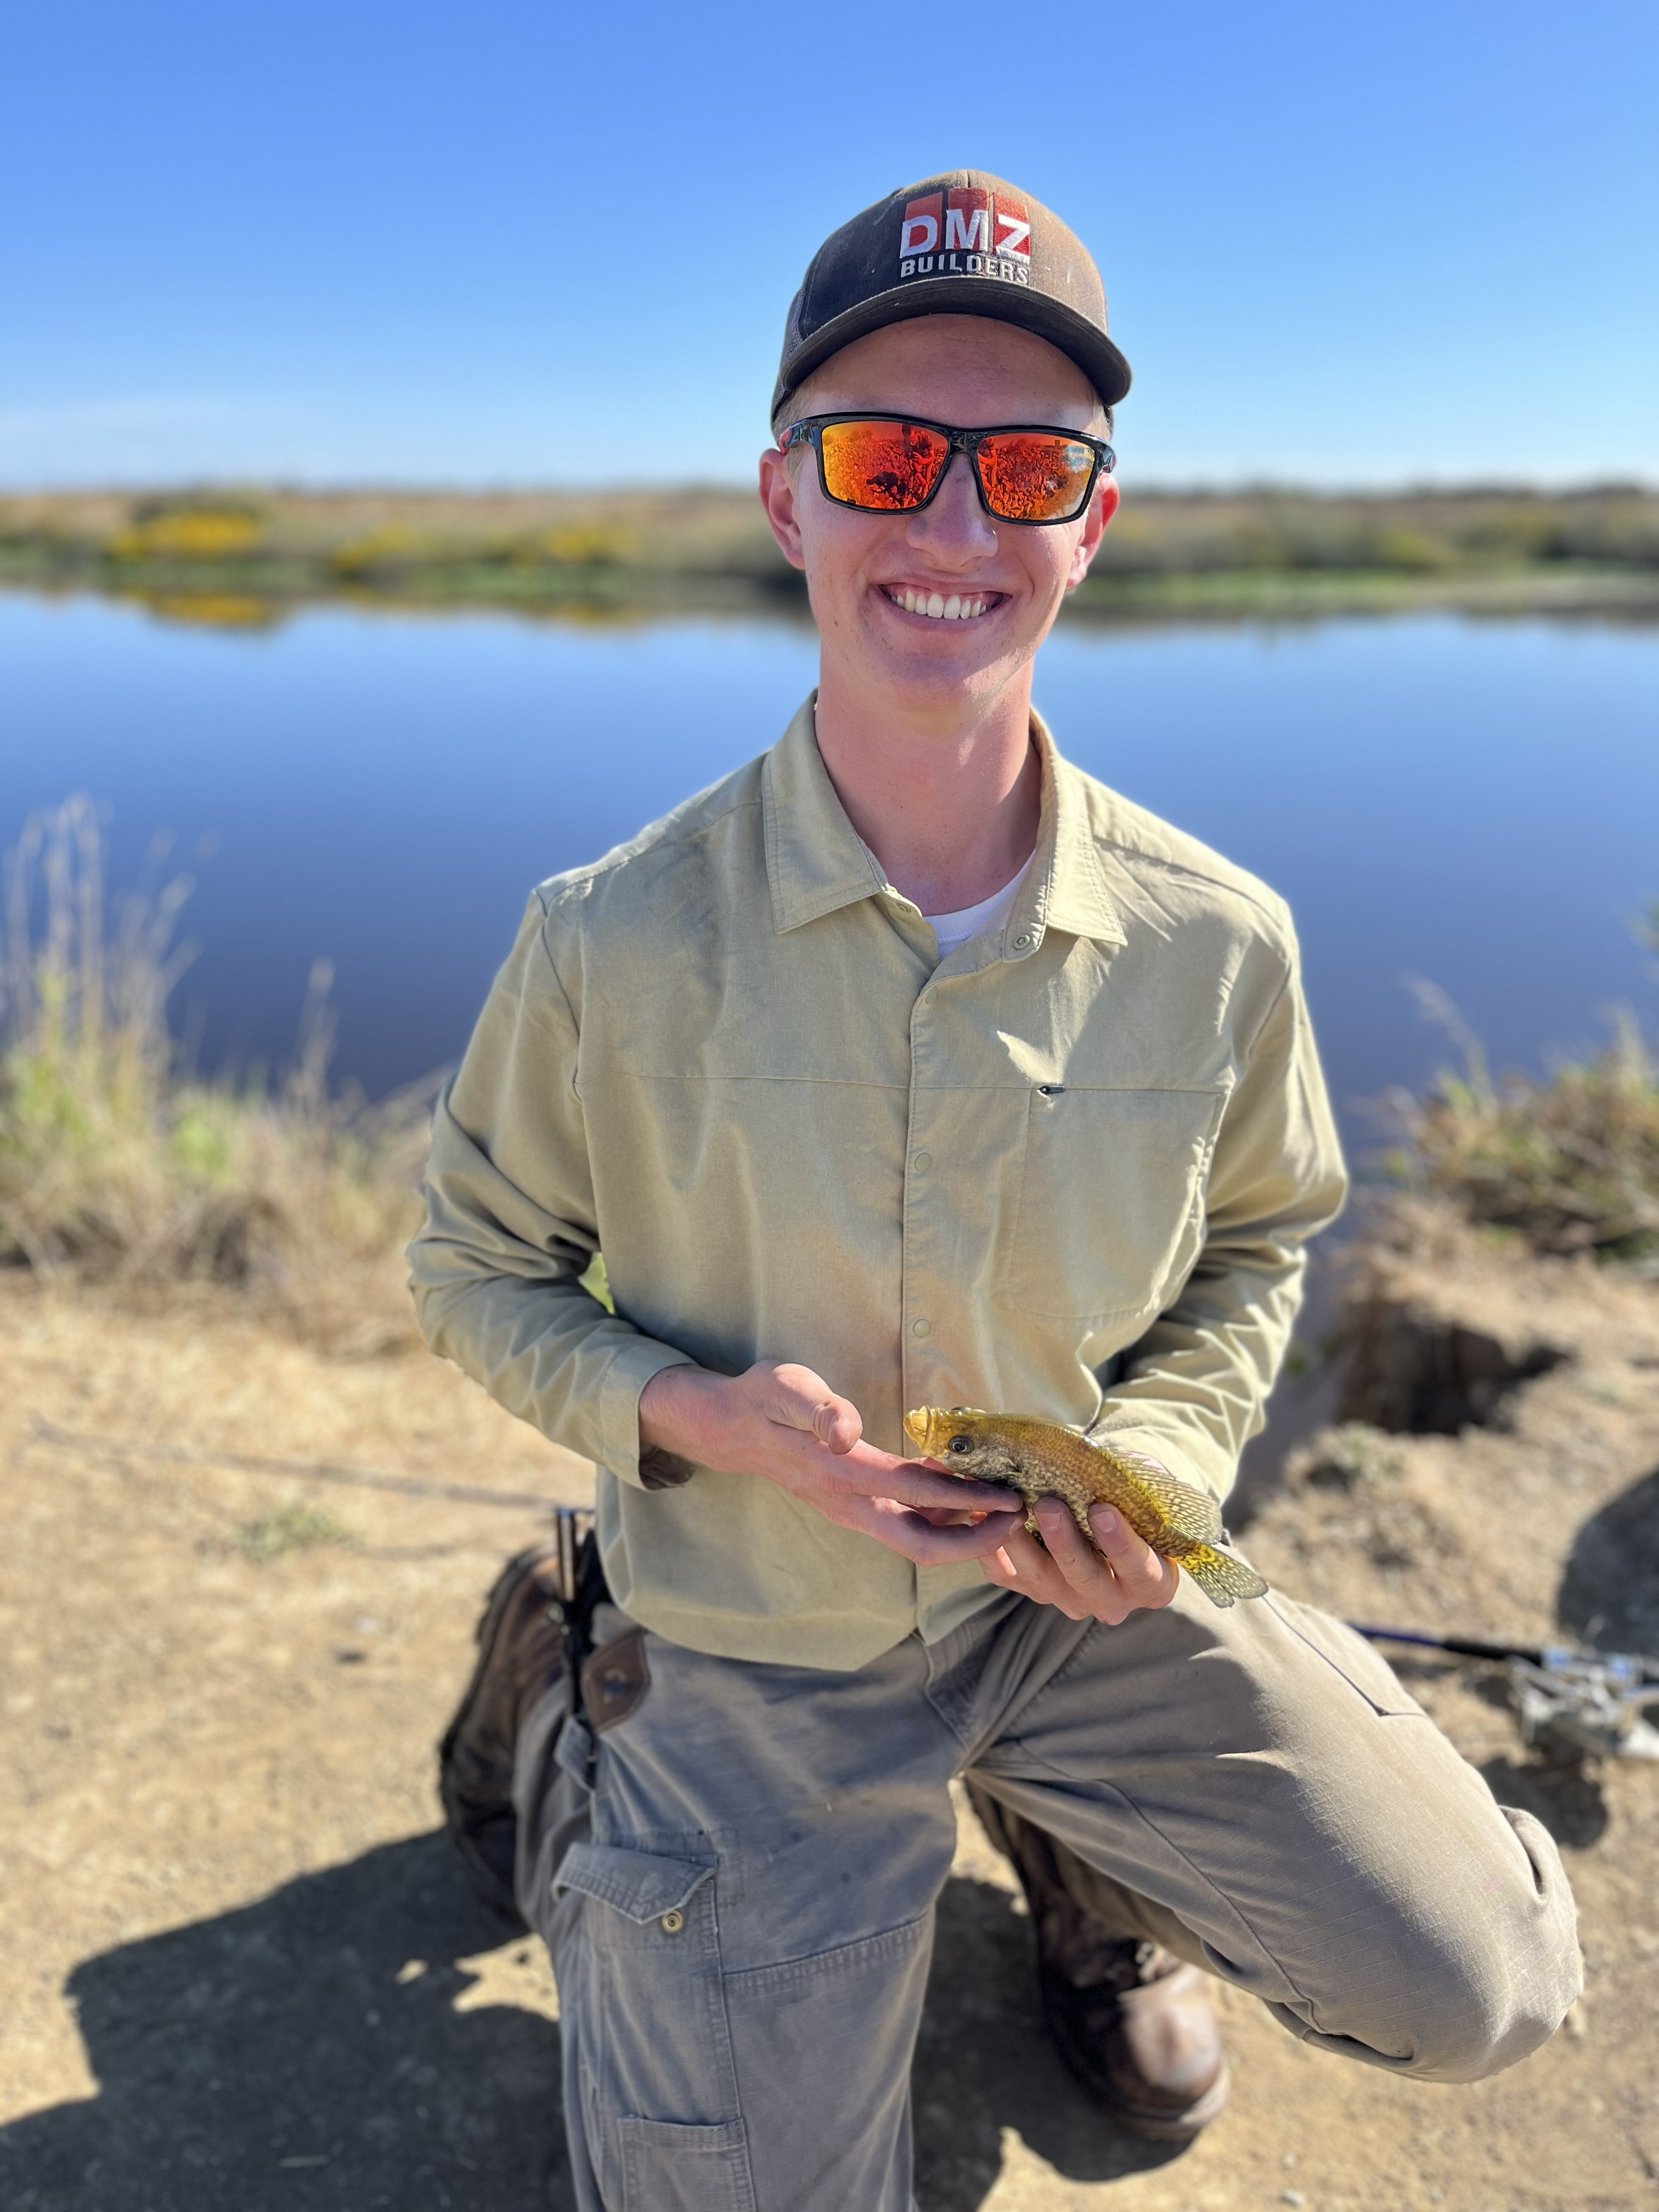
\includegraphics[width=0.85\textwidth]{holdfish.jpg} 
                    }

                    \caption{CAD model of the bellow}
                    \label{fig:bellow}
                \end{figure}



                \begin{table}[H]
                    \centering
                    \caption{Valve Specifications}
                    \label{tab:valve specification}
                    \begin{tabularx}{\textwidth}{l X l}
                        \toprule
                        \textbf{Requirements} & \textbf{Design Specification} & \textbf{Implemented Specification} \\
                        \midrule
                        Stroke &
                        $\leq$ \specStroke\ mm &
                        TODO: Insert actual stroke of mechanism
                        \\\addlinespace
                        Pressure &
                        $\Delta P \leq 68.95$~MPa &
                        TODO: Insert FOS or necessary par.
                        \\\addlinespace
                        Axial force &
                        \specPressureForceAxial N&
                        TODO: Insert force resisted
                        \\\addlinespace
                        Fluid compatibility &
                        "High" free energy of reaction with noble gas &
                        TODO: Insert material prop.
                        \\\bottomrule
                    \end{tabularx}
                \end{table}
            \subsubsection{Design Requirement Updates}
            \subsubsection{Current Implementation}
                The welded metal bellows transmits an axial stroke $\delta$ from an external actuator into a high-pressure hydrogen valve while maintaining zero leakage. The bellows must withstand internal pressure $P$, provide the required displacement without plastic deformation, and minimize actuator force demand.
                \\~\\
                Figure \ref{fig:bellow}, illustrates the valve assembly with the bellows highlighted. It is welded to the central valve housing and the valve stem, ensuring a leak-tight seal while permitting the necessary axial movement. The following equations address the key design parameters and constraints governing the selection of appropriate bellows geometry and material.
                Accounting for the spring force of the bellows is important for actuator sizing.
Let $K$ be the spring rate of the bellows, which depends on material properties, geometry, and convolution count $N$.
The spring force is proportional to deflection $\delta$.
\\~\\
Spring force:
$$F_s = K \delta = (630.46 \ \text{N/mm})(0.268 \ \text{mm}) \approx 168.96 \ \text{N}$$
The resulting spring force confirms that the stroke demand is well within the elastic operating range of the selected bellows.
The relatively high spring rate of $K = 630.46\ \text{N/mm}$ provides strong squirm resistance under pressure while still producing a manageable spring load given the small stroke $\delta$.
This balance between stiffness and stroke compliance is central to the optimized selection.
\\~\\
Total force required for actuation:
$$F_{total} = K \delta + F_{friction} \pm mg \approx 168.96 + F_{friction} \pm mg \ \text{N}$$
Since $\delta$ is very small, the spring force contribution is modest but nonetheless significant.
The term $F_{friction}$ accounts for any additional forces due to friction in the system, which is minimized through careful design and material selection.
The term $mg$ accounts for gravitational forces acting on the valve stem, which are minimal given the small mass of the stem.
Together, these contributions result in a low total actuation force demand that is easily achievable with a compact actuator.
\\~\\
Critical squirm pressure is the pressure at which the bellows becomes unstable and experiences lateral deformation.
This occurs when the bellows is unrestrained from sideways movement and the internal pressure exceeds the bellows' ability to maintain its shape.
Because the valve body provides lateral restraint, the bellows will not experience squirm, and the critical squirm pressure is therefore not a limiting factor in this design.
\\~\\
Burst pressure is the maximum pressure the bellows can withstand while laterally restrained.
The design is governed by the following relationship:
$$P_{operating} < P_{burst} \quad \Rightarrow \quad 68.95 \ \text{MPa} < 86.87 \ \text{MPa}$$
For this application, the bellows carries a safety factor of 1.26 against burst.
An optimized design targets a burst safety factor in this range, as too low a factor risks failure under overpressure events, while too high a factor necessitates a larger, stiffer bellows that increases spring load and actuator demand.
                \begin{table}[H]
                    \centering
                    \caption{Bellows Parameters}
                    \label{tab:bellows_parameters}
                    \begin{tabularx}{\textwidth}{l X l}
                        \toprule
                        \textbf{Parameter} & \textbf{Description} & \textbf{Value} \\
                        \midrule
                        $D_o$ &
                        Outside convolution diameter &
                        4.826 mm
                        \\\addlinespace
                        $D_i$ &
                        Inside convolution diameter &
                        2.616 mm
                        \\\addlinespace
                        $t$ &
                        Wall thickness &
                        0.183 mm
                        \\\addlinespace
                        $L$ &
                        Convolution free length &
                        4.191 mm
                        \\\addlinespace
                        $A$ &
                        Effective area &
                        $10.84 \ \text{mm}^2$
                         \\\addlinespace
                        $N$ &
                        Number of convolutions &
                        7
                        \\\addlinespace
                        $P_{burst}$ &
                        Burst pressure &
                        86.87 MPa
                        \\\addlinespace
                        $k$ &
                        Spring rate &
                        630.46 N/mm
                        \\\addlinespace
                        Material &
                        Hydrogen Compatible &
                        Inconel 718
                        \\\bottomrule
                    \end{tabularx}
                \end{table}

    
% ============================================================================
% SECTION 4: PRELIMINARY BILL OF MATERIALS
% ============================================================================
% GRADING: Section V — 10 points
%   "All parts included, each part belongs to a sub system,
%    accurate costs, all info included"
%
% TEMPLATE GUIDANCE:
%   - TABLE FORMAT (mandatory)
%   - Include: part numbers, part names, quantity, material,
%     purchased vs fabricated, supplier name/part number if purchased
%   - For fabricated parts: size and cost of raw material
%   - Include any special tooling that must be purchased
%   - Must be complete enough to release your budget for Spring quarter
%
% ESTIMATED LENGTH: 1-2 pages
%
% TIP: The longtable environment is used here because the BOM may
% span multiple pages. Regular tabular would break across pages poorly.
% ============================================================================

\chapter{Preliminary Bill of Materials}
\label{sec:bom}

%--- BEGIN CONTENT ---

\todo{Write a brief introductory paragraph explaining the BOM structure
and the total estimated project cost.}

% --- The BOM Table ---
% Using longtable so it can span multiple pages if needed.
% Column specification:
%   c = centered, l = left-aligned, r = right-aligned
%   p{width} = paragraph column with fixed width (for wrapping long text)

\begin{longtable}{c l p{1.8in} c c c r}

    % --- Table Header (appears on every page) ---
    \caption{Preliminary Bill of Materials and Cost Estimate}
    \label{tab:bom} \\

    \toprule
    \textbf{Item} &
    \textbf{Part Name} &
    \textbf{Description / Supplier} &
    \textbf{Qty} &
    \textbf{Material} &
    \textbf{P/F} &
    \textbf{Cost (\$)} \\
    \midrule
    \endfirsthead

    % --- Continuation header (on subsequent pages) ---
    \multicolumn{7}{c}{\small\itshape (continued from previous page)} \\
    \toprule
    \textbf{Item} &
    \textbf{Part Name} &
    \textbf{Description / Supplier} &
    \textbf{Qty} &
    \textbf{Material} &
    \textbf{P/F} &
    \textbf{Cost (\$)} \\
    \midrule
    \endhead

    % --- Footer on all pages except last ---
    \midrule
    \multicolumn{7}{r}{\small\itshape (continued on next page)} \\
    \endfoot

    % --- Footer on the last page ---
    \midrule
    \multicolumn{6}{r}{\textbf{Estimated Total:}} &
    \textbf{\todo{XX.XX}} \\
    \bottomrule
    \endlastfoot

    % ---- Subsystem: Actuator ----
    \multicolumn{7}{l}{\textbf{Actuator Subsystem}} \\
    \midrule
    1 & \todo{Part name} & \todo{Description / McMaster \#} & \todo{1} & \todo{Steel} & P & \todo{XX.XX} \\
    2 & \todo{Part name} & \todo{Description} & \todo{1} & \todo{Al 6061} & F & \todo{XX.XX} \\
    \addlinespace

    % ---- Subsystem: Valve ----
    \multicolumn{7}{l}{\textbf{Valve Subsystem}} \\
    \midrule
    3 & \todo{Part name} & \todo{Description} & \todo{1} & \todo{SS 316} & P & \todo{XX.XX} \\
    4 & \todo{Part name} & \todo{Description} & \todo{1} & \todo{Brass} & F & \todo{XX.XX} \\
    \addlinespace

    % ---- Subsystem: Housing ----
    \multicolumn{7}{l}{\textbf{Housing \& Interface}} \\
    \midrule
    5 & \todo{Part name} & \todo{Description} & \todo{1} & \todo{SS 316} & F & \todo{XX.XX} \\
    6 & \todo{Part name} & \todo{Description} & \todo{2} & \todo{Viton} & P & \todo{XX.XX} \\
    \addlinespace

    % ---- Subsystem: Fasteners & Misc ----
    \multicolumn{7}{l}{\textbf{Fasteners \& Miscellaneous}} \\
    \midrule
    7 & \todo{Part name} & \todo{Description} & \todo{10} & \todo{Steel} & P & \todo{XX.XX} \\
    \addlinespace

    % ---- Tooling (if any) ----
    \multicolumn{7}{l}{\textbf{Special Tooling}} \\
    \midrule
    8 & \todo{Tooling item} & \todo{Description} & \todo{1} & --- & P & \todo{XX.XX} \\

\end{longtable}

% P/F Key
\textbf{Key:} P = Purchased, F = Fabricated

\todo{Add any notes about budget constraints, contingency funds, or
items awaiting price quotes.}

%--- END CONTENT ---


% ============================================================================
% SECTION 5: PROJECT MANAGEMENT INFORMATION
% ============================================================================
% GRADING: Section VI — 15 points total
%   6.1) Appropriate tasks identified over 2 quarters (5.0 pts)
%   6.2) Updated Gantt chart for 2 quarters (5.0 pts)
%   6.3) Critical path method (CPM) analysis (5.0 pts)
%
% TEMPLATE GUIDANCE:
%   - Task list must be specific to YOUR project and design
%   - Gantt chart must span BOTH quarters (Fall through Spring)
%   - CPM must be in graphical format with a paragraph description
%   - If permits or PE sign-offs are needed, note them here
%
% ESTIMATED LENGTH: 3-4 pages (could be longer)
% ============================================================================

\chapter{Project Management Information}
\label{sec:project_management}


% --- 5.1: Task List ---
\section{Updated Task List}
\label{subsec:task_list}

%--- BEGIN CONTENT ---

\todo{Provide a detailed task list. Organize by phase or subsystem.
Must include:
\begin{itemize}
    \item Technical tasks (design, fabrication, testing)
    \item Deliverables for class (reports, presentations)
    \item Team and stakeholder meetings
    \item Procurement / ordering deadlines
\end{itemize}}

% Example task table:
\begin{table}[H]
    \centering
    \caption{Updated task list for Winter and Spring quarters.}
    \label{tab:task_list}
    \begin{tabularx}{\textwidth}{c X l l}
        \toprule
        \textbf{\#} & \textbf{Task Description} & \textbf{Owner(s)} & \textbf{Deadline} \\
        \midrule
        1 & Finalize engineering drawings & \todo{Name(s)} & \todo{Date} \\
        2 & Order raw materials & \todo{Name(s)} & \todo{Date} \\
        3 & Machine actuator housing & \todo{Name(s)} & \todo{Date} \\
        4 & Assemble prototype & \todo{Name(s)} & \todo{Date} \\
        5 & Conduct thermal testing & \todo{Name(s)} & \todo{Date} \\
        6 & Conduct pressure testing & \todo{Name(s)} & \todo{Date} \\
        7 & \todo{Add more tasks} & & \\
        \bottomrule
    \end{tabularx}
\end{table}

%--- END CONTENT ---


% --- 5.2: Gantt Chart ---
\section{Gantt Chart}
\label{subsec:gantt}

%--- BEGIN CONTENT ---

\todo{Insert your Gantt chart. This is typically created in Excel, MS Project,
or a similar tool and exported as an image.}

\begin{figure}[H]
    \centering
    % \includegraphics[width=\textwidth]{gantt_chart.png}

    % Placeholder:
    \fbox{\parbox[c][3in]{\textwidth}{%
        \centering\Large\color{gray}%
        [Gantt Chart --- Two Quarters]\\[6pt]
        \normalsize Export from Excel/MS Project as PNG or PDF.\\
        Must span Winter 2026 through Spring 2026.\\
        Show current progress with a vertical ``today'' line.
    }}

    \caption{Updated Gantt chart spanning Winter and Spring quarters.
    The vertical dashed line indicates the current date.}
    \label{fig:gantt}
\end{figure}

\todo{Write a paragraph interpreting the Gantt chart. Highlight key
milestones and any tasks that are ahead of or behind schedule.}

%--- END CONTENT ---


% --- 5.3: Critical Path Method (CPM) Analysis ---
\section{Critical Path Method (CPM) Analysis}
\label{subsec:cpm}

%--- BEGIN CONTENT ---

\todo{Insert your CPM network diagram. This must be in GRAPHICAL format.}

\begin{figure}[H]
    \centering
    % \includegraphics[width=\textwidth]{cpm_diagram.png}

    % Placeholder:
    \fbox{\parbox[c][3in]{\textwidth}{%
        \centering\Large\color{gray}%
        [CPM Network Diagram]\\[6pt]
        \normalsize Show tasks as nodes, dependencies as arrows.\\
        Highlight the critical path in red or bold.\\
        Include earliest start/finish and latest start/finish times.
    }}

    \caption{Critical path method (CPM) network diagram. The critical
    path is highlighted in red.}
    \label{fig:cpm}
\end{figure}

\todo{Write a paragraph describing:
\begin{itemize}
    \item What the critical path is (list the tasks)
    \item Total project duration along the critical path
    \item Which tasks have float (slack time)
    \item What the analysis tells you about risk and scheduling
    \item Any mitigation strategies for critical-path delays
\end{itemize}}

%--- END CONTENT ---


% ============================================================================
% SECTION 6: CITED REFERENCES
% ============================================================================
% GRADING: Part of Section I (General Considerations)
%   "Appropriate technical references" and "professional in appearance"
%
% TEMPLATE GUIDANCE:
%   - Use citations as appropriate for technical writing
%   - Cite other's work, supporting assumptions, technical data
%   - Use a consistent format (IEEE, APA, MLA — pick one)
%
% HOW THIS WORKS IN LATEX:
%   Option A (recommended): Use BibTeX with a .bib file.
%   Option B (simpler): Use thebibliography environment (shown below).
%
%   For Option A, create a file called "references.bib" with entries like:
%     @article{bon2025,
%       author  = {Bon, Bradley},
%       title   = {Passive Flow Control for Hydrogen Systems},
%       journal = {Sandia Technical Report},
%       year    = {2025}
%     }
%   Then cite with: \cite{bon2025}
%   And compile with: pdflatex -> bibtex -> pdflatex -> pdflatex
% ============================================================================

\chapter{Cited References}
\label{sec:references}

% --- Option B: Manual bibliography (simpler, no .bib file needed) ---
% Each \bibitem{key} creates a reference. Cite with \cite{key} in text.
%
% The [99] tells LaTeX the widest label will be two digits.
% Change to [9] if you have fewer than 10 references.

\begin{thebibliography}{99}

    \bibitem{ref_sandiaprompt}
    B.\ Bon,
    ``Passive Temperature Compensation Device --- Project Prompt,''
    Sandia National Laboratories, SAND2025-15446O, 2025.

    \bibitem{ref_placeholder2}
    \todo{Add reference: textbook, paper, or technical standard}

    \bibitem{ref_placeholder3}
    \todo{Add reference: material property data source}

    \bibitem{ref_placeholder4}
    \todo{Add reference: relevant prior work or patent}

    % Add more \bibitem entries as needed.
    % In the body text, cite as: \cite{ref_sandiaprompt}

\end{thebibliography}


% ============================================================================
% APPENDICES
% ============================================================================
% TEMPLATE GUIDANCE:
%   - Label and title every appendix
%   - You MUST refer to each appendix in the body of the report
%   - Include: working drawings, product sheets, price quotes,
%     updated requirements table, scoring matrices, etc.
%
% IMPORTANT: Appendices don't count toward estimated page lengths
% of other sections, so put detailed tables and drawings here.
% ============================================================================

\newpage
\begin{appendices}


% --- Appendix A: Updated Design Requirements ---
\section{Updated Design Requirements}
\label{app:requirements}

\todo{Include the final, updated requirements table here. This should
reflect any changes discussed in Section~\ref{subsec:req_updates}.
Organize by category (system-level, actuator, valve, housing, etc.).
Include the subsystem-level rolldown specifications.}


% --- Appendix B: Concept Screening and Scoring Matrices ---
\section{Concept Screening and Scoring Matrices}
\label{app:scoring}

\todo{Include the screening matrix and weighted scoring matrix from
your concept selection process. These were referenced in
Section~\ref{subsec:selection_criteria}.}

% TIP: If your matrices are in Excel (Concept_Screening_Scoring_Matrix.xlsx),
% export them as images and include them here:
%
% \insertfigure{0.9}{screening_matrix.png}{Concept screening matrix
%   for actuator subsystem.}{fig:screening_matrix}
%
% \insertfigure{0.9}{scoring_matrix.png}{Weighted scoring matrix
%   for actuator subsystem.}{fig:scoring_matrix}


% --- Appendix C: Engineering Drawing Package ---
\section{Engineering Drawing Package}
\label{app:drawings}

\todo{Include complete assembly, sub-assembly, and part drawings.
Part drawings must include dimensions and tolerances for all
parts that will be MANUFACTURED (not purchased).
Follow proper engineering drawing practices.

Organize as:
\begin{enumerate}
    \item Full system assembly drawing
    \item Actuator sub-assembly drawing
    \item Valve sub-assembly drawing
    \item Housing sub-assembly drawing
    \item Individual part drawings (manufactured parts only)
\end{enumerate}

Each drawing should be on its own page for clarity.
Label as Figure A.1, A.2, etc.}


% --- Appendix D: Product Data Sheets and Price Quotes ---
\section{Product Data Sheets and Price Quotes}
\label{app:datasheets}

\todo{Include manufacturer spec sheets for all purchased components.
Include price quotes or screenshots of supplier pricing.
This supports the Bill of Materials in Section~\ref{sec:bom}.}


% --- Appendix E: Detailed Calculations ---
\section{Detailed Calculations}
\label{app:calculations}

\todo{If your calculations in Section~\ref{subsec:calculations} were
summarized for brevity, include the full derivations and spreadsheet
screenshots here. Reference Performance\_Relationship.xlsx and
Thermal\_Expansion.xlsx data as appropriate.}


\end{appendices}


% ============================================================================
% END OF DOCUMENT
% ============================================================================
% FINAL CHECKLIST BEFORE SUBMISSION:
%
%   [ ] All TODO items have been replaced with actual content
%   [ ] All figures have real images (no gray placeholders remaining)
%   [ ] All figures and tables are referenced in the text
%   [ ] All appendices are referenced in the body of the report
%   [ ] Table of Contents page numbers are correct (compile twice!)
%   [ ] Acronyms defined on first use
%   [ ] Units are consistent (SI preferred, with imperial conversions if needed)
%   [ ] Spell check completed
%   [ ] Grammar check completed
%   [ ] All team members have reviewed the final document
%   [ ] PDF is under any file size limits
%
% GRADING SELF-CHECK:
%   [ ] I.   General Considerations (20 pts) — Format, presentation, TOC, readability
%   [ ] II.  Abstract (10 pts) — 300-500 words, clear, technically accurate
%   [ ] III. System Architecture (20 pts) — Criteria, drawings, description
%   [ ] IV.  Discussion (25 pts) — Requirements, subsystems, calculations
%   [ ] V.   Bill of Materials (10 pts) — Complete, accurate, in table format
%   [ ] VI.  Project Management (15 pts) — Tasks, Gantt (2 quarters), CPM
% ============================================================================

\end{document}